\documentclass[tikz,border=5]{standalone}
\usepackage[T1]{fontenc}
\usepackage{amsmath,amssymb,enumerate, amsthm}
\usepackage[dvipsnames]{xcolor}
\usepackage{tikz}
\usetikzlibrary{shapes}
\usepackage[many]{tcolorbox}
\usetikzlibrary{decorations.pathreplacing}
\usepackage{colortbl}
\tikzset{
	mystyle/.style={line width = 1.5pt, color = red!70!black}
}

\begin{document}

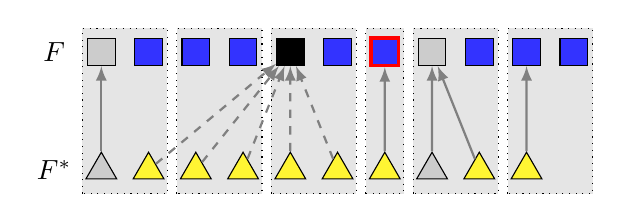
\begin{tikzpicture}[scale=0.6,
		opt/.style={shape=regular polygon,regular polygon sides = 3,draw=black,minimum size=0.45cm,inner sep = 0pt},
		local/.style={shape=rectangle, draw=black,minimum size= 0.35cm},
		swap/.style={fill=gray!20!white,dotted}
]
\pgfset{
  foreach/parallel foreach/.style args={#1in#2via#3}{evaluate=#3 as #1 using {{#2}[#3-1]}},
}
	\def \n {4}
	
	\draw[swap] (0.6,-0.5) rectangle (2.4,3);
	\draw[swap] (2.6,-0.5) rectangle (4.4,3);	
	\draw[swap] (4.6,-0.5) rectangle (6.4,3);	
	\draw[swap] (6.6,-0.5) rectangle (7.4,3);
	\draw[swap] (7.6,-0.5) rectangle (9.4,3);	
	\draw[swap] (9.6,-0.5) rectangle (11.4,3);		

	\def \cc {black!20}
	\def \candc {blue!80!white}
	\def \srgtc {black}
	\def \srgtoc {yellow!80}
	
	\def \colorlistf{"\cc","\candc","\candc","\candc","\srgtc","\candc","\candc","\cc","\candc","\candc","\candc"}	
	\def \colorlisto{"\cc","\srgtoc","\srgtoc","\srgtoc","\srgtoc","\srgtoc","\srgtoc","\cc","\srgtoc","\srgtoc"}	


	\foreach \i [parallel foreach=\c in \colorlisto via \i] in {1,...,10}{
		\node [opt,fill=\c] (o\i) at (\i,0) {};
	}
	\foreach \i [parallel foreach=\c in \colorlistf via \i] in {1,...,6,8,9,10,11}{
		\node [local,fill=\c] (f\i) at (\i,2.5) {};
	}
	\node [local,fill=\candc,draw = red,very thick] (f7) at (7,2.5) {};
	
	\draw (o1) edge[->,>=latex,gray,thick] (f1);
	\draw (o2) edge[->,>=latex,gray,thick,dashed] (f5);
	\draw (o3) edge[->,>=latex,gray,thick,dashed] (f5);
	\draw (o4) edge[->,>=latex,gray,thick,dashed] (f5);
	\draw (o5) edge[->,>=latex,gray,thick,dashed] (f5);
	\draw (o6) edge[->,>=latex,gray,thick,dashed] (f5);
	\draw (o7) edge[->,>=latex,gray,thick] (f7);
	\draw (o8) edge[->,>=latex,gray,thick] (f8);
	\draw (o9) edge[->,>=latex,gray,thick] (f8);
	\draw (o10) edge[->,>=latex,gray,thick] (f10);	

	\node at (0,0) {$F^*$};
	\node at (0,2.5) {$F$};	

\end{tikzpicture}

\end{document}